%%
%% This is file `sample-sigconf.tex',
%% generated with the docstrip utility.
%%
%% The original source files were:
%%
%% samples.dtx  (with options: `sigconf')
%% 
%% IMPORTANT NOTICE:
%% 
%% For the copyright see the source file.
%% 
%% Any modified versions of this file must be renamed
%% with new filenames distinct from sample-sigconf.tex.
%% 
%% For distribution of the original source see the terms
%% for copying and modification in the file samples.dtx.
%% 
%% This generated file may be distributed as long as the
%% original source files, as listed above, are part of the
%% same distribution. (The sources need not necessarily be
%% in the same archive or directory.)
%%
%%
%% Commands for TeXCount
%TC:macro \cite [option:text,text]
%TC:macro \citep [option:text,text]
%TC:macro \citet [option:text,text]
%TC:envir table 0 1
%TC:envir table* 0 1
%TC:envir tabular [ignore] word
%TC:envir displaymath 0 word
%TC:envir math 0 word
%TC:envir comment 0 0
%%
%%
%% The first command in your LaTeX source must be the \documentclass command.
\documentclass[sigconf]{acmart}

%%
%% \BibTeX command to typeset BibTeX logo in the docs
\AtBeginDocument{%
  \providecommand\BibTeX{{%
    \normalfont B\kern-0.5em{\scshape i\kern-0.25em b}\kern-0.8em\TeX}}}

%% Rights management information.  This information is sent to you
%% when you complete the rights form.  These commands have SAMPLE
%% values in them; it is your responsibility as an author to replace
%% the commands and values with those provided to you when you
%% complete the rights form.
\setcopyright{acmcopyright}
\copyrightyear{2021}
\acmYear{2021}
\acmDOI{10.1145/1122445.1122456}

%% These commands are for a PROCEEDINGS abstract or paper.
% \acmConference[Woodstock '18]{Woodstock '18: ACM Symposium on Neural
%   Gaze Detection}{June 03--05, 2018}{Woodstock, NY}
% \acmBooktitle{Woodstock '18: ACM Symposium on Neural Gaze Detection,
%   June 03--05, 2018, Woodstock, NY}
% \acmPrice{15.00}
% \acmISBN{978-1-4503-XXXX-X/18/06}


%%
%% Submission ID.
%% Use this when submitting an article to a sponsored event. You'll
%% receive a unique submission ID from the organizers
%% of the event, and this ID should be used as the parameter to this command.
%%\acmSubmissionID{123-A56-BU3}

%%
%% The majority of ACM publications use numbered citations and
%% references.  The command \citestyle{authoryear} switches to the
%% "author year" style.
%%
%% If you are preparing content for an event
%% sponsored by ACM SIGGRAPH, you must use the "author year" style of
%% citations and references.
%% Uncommenting
%% the next command will enable that style.
%%\citestyle{acmauthoryear}

\usepackage{xeCJK}
\setCJKmainfont{[NotoSansTC-Regular.otf]}
\usepackage{hyperref}
\usepackage{xurl}
\usepackage{multirow}
\usepackage{diagbox}
\usepackage{float}

\definecolor{barblue}{RGB}{153,204,254}
\definecolor{groupblue}{RGB}{51,102,254}
\definecolor{linkred}{RGB}{165,0,33} 

%%
%% end of the preamble, start of the body of the document source.
\begin{document}

%%
%% The "title" command has an optional parameter,
%% allowing the author to define a "short title" to be used in page headers.
\title{Exploring Parallel MCTS on Chess Game}

%%
%% The "author" command and its associated commands are used to define
%% the authors and their affiliations.
%% Of note is the shared affiliation of the first two authors, and the
%% "authornote" and "authornotemark" commands
%% used to denote shared contribution to the research.

\author{曾正豪 0716325}
\affiliation{%
  \institution{CS NYCU}
  \city{Hsinchu}
  \country{Taiwan}}

\author{張宸愷 0710018}
\affiliation{%
  \institution{EECSHP NYCU}
  \city{Hsinchu}
  \country{Taiwan}}




%%
%% By default, the full list of authors will be used in the page
%% headers. Often, this list is too long, and will overlap
%% other information printed in the page headers. This command allows
%% the author to define a more concise list
%% of authors' names for this purpose.
% \renewcommand{\shortauthors}{Trovato and Tobin, et al.}

%%
%% The abstract is a short summary of the work to be presented in the
%% article.
\begin{abstract}
  A project proposal for the course `Parallel Programming Fall 2021'.
  We decided to explore the parallelization of Monte Carlo Tree Search using the techniques and knowledge we have learned in this course. We will use quantitative benchmarks to compare different approaches to solve this kind of parallelization. 
\end{abstract}

%%
%% The code below is generated by the tool at http://dl.acm.org/ccs.cfm.
%% Please copy and paste the code instead of the example below.
%%

% [TODO] css insert here


%%
%% Keywords. The author(s) should pick words that accurately describe
%% the work being presented. Separate the keywords with commas.
\keywords{MCTS, parallel programming, Pthreads, CUDA, Chess}

%% A "teaser" image appears between the author and affiliation
%% information and the body of the document, and typically spans the
%% page.
\begin{teaserfigure}
  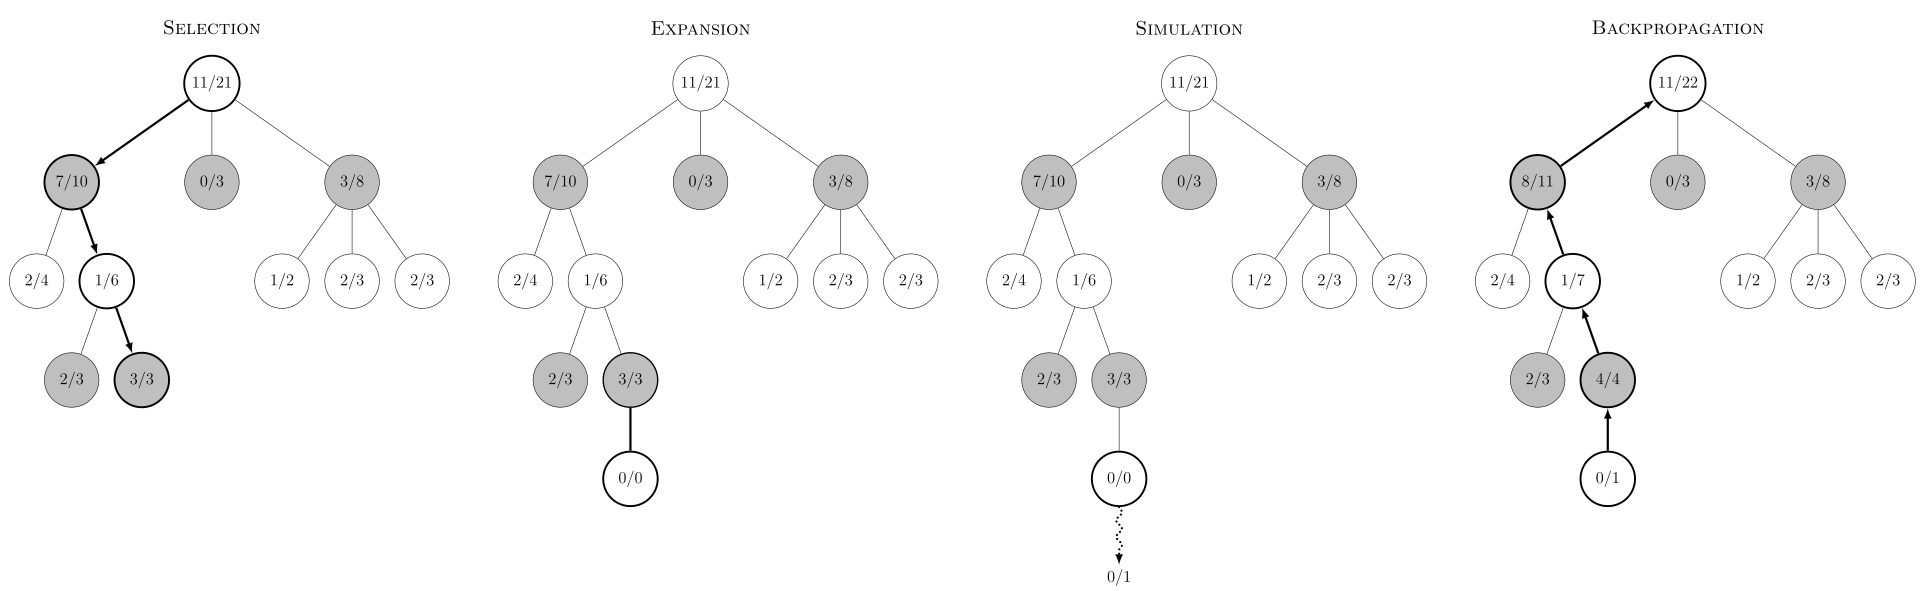
\includegraphics[width=\textwidth]{MCTS-steps.png}
  \caption{Illustration for a single step of MCTS}
  \Description{The workings of MCTS}
\label{fig:teaser}
\end{teaserfigure}

%%
%% This command processes the author and affiliation and title
%% information and builds the first part of the formatted document.
\maketitle

\section{Introduction}
`Monte Carlo Tree Search', abbreviated in this text from now on as MCTS, is a probability sampling based tree search method for many applications. One of the most famous application of MCTS is AlphaGO~\cite{alphaGo}. It uses MCTS with 2 other neural networks to play Go. An early version of AlphaGo was tested on hardware with various numbers of CPUs and GPUs, running in asynchronous or distributed mode. It was tested with search threads from 12 to 64, number of CPUs from 48 to 1920, and number of GPUs from 1 to 280. And in 2016, it changed to use TPUs (tensor processing units) as its computing unit. In recent years, it keeps beating many go players. Overall, MCTS is an algorithm that can be highly parallelized because of the high number of simulations. Hence, we decided to use MCTS as the topic of our final project.

\section{Statement of problem}
One of our teammates had taken the course AI capstone, and during that course he had been doing a final project about playing a 3D version of connect-4 using upper confidence bound MCTS, i.e. UCB-MCTS. He noticed that when he uses root parallelization, the performance of the MCTS decreases dramatically. The multithreaded version with 8 threads didn't even manage to beat the single-threaded one. Thus, we want to explore further on why it didn’t perform better and try to improve the multithreaded performance. The teammate's guess is that it's because of false sharing. 

\section{Proposed approaches}
\subsection{Overall design}
\begin{figure}[h]
  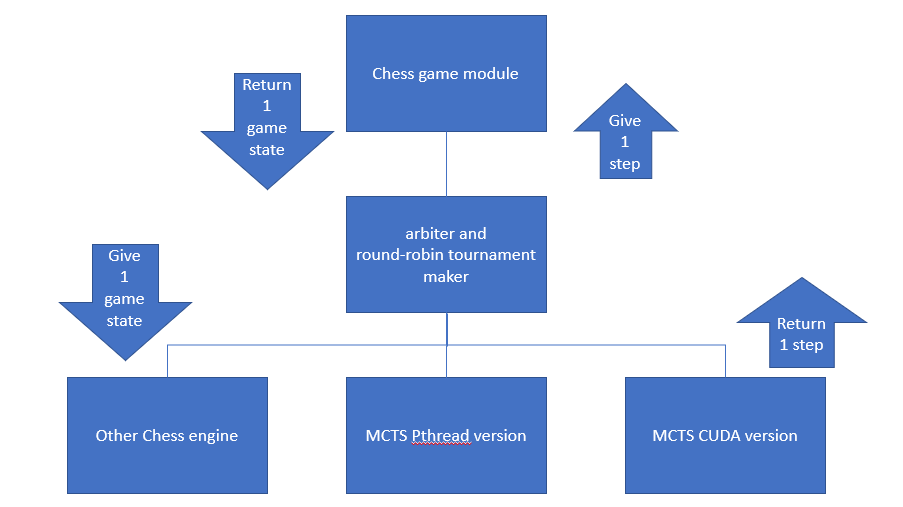
\includegraphics[width=8.5cm]{system-design.png}
  \caption{Our system diagram}
  \Description{system design}
\label{fig:system_design}
\end{figure}
Figure~\ref{fig:system_design} is our system design. Component descriptions:
\begin{itemize}
  \item Chess game module: Deal with the game state of Chess, once it receives a legal move, it will change its game state and return it.
  \item Arbiter and round-robin tournament maker: It will coordinate the game player and the game module. It checks if one move is legal and whether the game ends.
  \item 3 MCTS versions: To calculate the best move next. It will receive a game state and return its best move. The difference between these 3 versions is their parallel approach.
  \item Additional: Maybe we will compete with other Chess engines to see the performance pitted against other state of the art, if we have enough time.
\end{itemize}
The performance of each method will depend on the games won, and the total amount of expanded nodes. 

\subsection{parallelization details}
There are four ways to parallelize traditional UCB-MCTS mentioned in~\cite{guillaumeMCTS}, and illustrated in figure~\ref{fig:mcts_parallel}. Leaf parallelization, root parallelization, tree parallelization with global mutex, and tree parallelization with local mutex. 
\begin{figure}[h]
  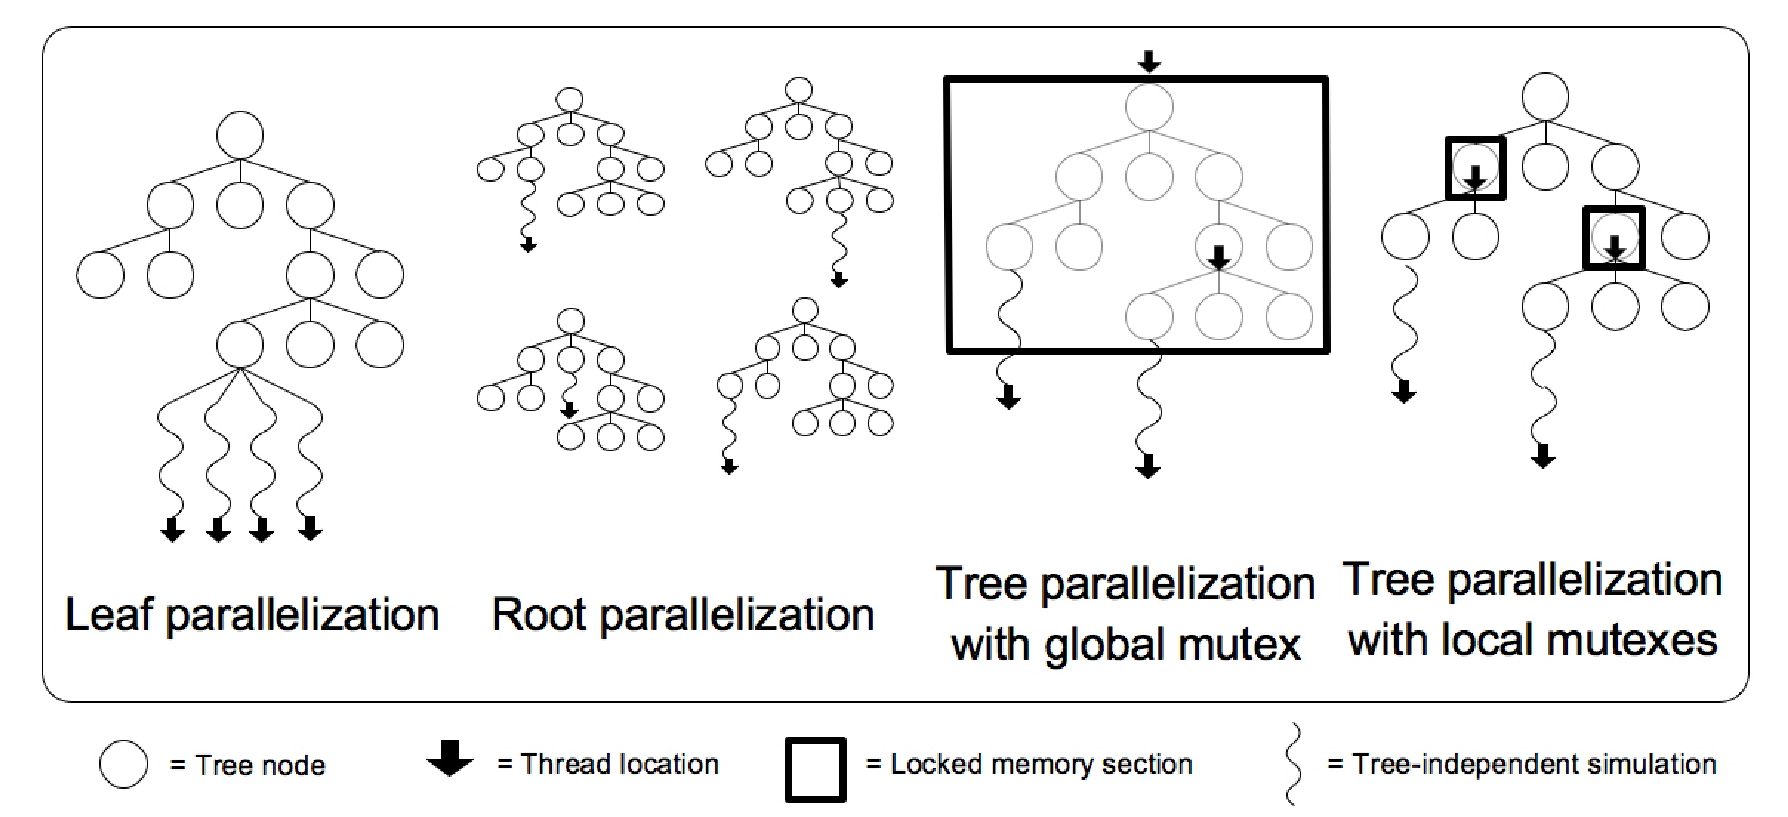
\includegraphics[width=8.5cm]{MCTS-parallel.png}
  \caption{Ways of parallelizing MCTS}
  \Description{Parallel MCTS}
\label{fig:mcts_parallel}
\end{figure}


\section{Language selection}
We will use C++ as our main programming language, together with Pthreads and CUDA, since we want to compare the performance of CPU and GPU on parallel programs.

\section{Related work}

A pretty detailed work~\cite{liu2020effective}. Different methods for enhancing the capability of MCTS on board games were explored in~\cite{weigel2017monte}.~\cite{guillaumeMCTS}\cite{weigel2017monte} also outlined some of the parallelization techniques for MCTS, root parallelization, leaf parallelization, and tree parallelization, etc.

\section{Expected results}
When using tree parallelization, there will be two methods. One is we use a global mutex to protect all the nodes in the tree. The other is to give each node a mutex. The former will be much slower because many threads are contending for a single lock, while the latter will use significantly more memory because each node has a lock, but the performance will be better. \\


\section{Timetable}
Below are the rough due dates for the individual components of our project. 
\begin{itemize}
  \item 10/27 proposal
  \item 11/05 chess engine wrapper, and game module
  \item 11/20 Pthread version
  \item 12/10 CUDA version
  \item 12/17 Performance analysis
  \item 12/31 Finalize report and source code
  
\end{itemize}


\section{Appendices}
%%
%% The next two lines define the bibliography style to be used, and
%% the bibliography file.
\bibliographystyle{ACM-Reference-Format}
\bibliography{reference}

%%
%% If your work has an appendix, this is the place to put it.
\appendix

\section{Online Resources}
% \begin{verbatim*}
%   https://en.wikipedia.org/wiki/Monte_Carlo_tree_search
% \end{verbatim*}
\begin{enumerate}
  \item Monte Carlo tree search (\url{https://en.wikipedia.org/wiki/Monte_Carlo_tree_search})
\end{enumerate}


\end{document}
\endinput
%%
%% End of file `sample-sigconf.tex'.
